\chapter{System Design and Methodology}

This chapter describes the research methodology, the system's domain boundaries, its architecture, and the algorithms and tools that underpin it.

\section{Research Design}

The research methodology follows a constructive research approach, also known as design science \cite{hevner2004design}, where a software artifact is systematically designed, built, and empirically evaluated to address a practical problem---in this case, cloud architecture recommendation and validation. This approach emphasizes iterative cycles of design, software development, and quantitative/qualitative assessment. In the context of this thesis, the constructive artifact is the Agentic AI Framework, and the empirical evaluation is conducted using the quantitative NLP metrics detailed in Chapter 5.

\section{System Domain: Multi-Cloud Environment (AWS and Azure)}

The system domain covers the two leading public cloud providers: Amazon Web Services (AWS) and Microsoft Azure. Both vendors expose hundreds of interrelated services that frequently overlap in purpose but differ in API design, pricing structures, and operational characteristics. A containerised compute workload, for instance, can target Amazon ECS or EKS on AWS, or Azure Container Apps and AKS on Azure; the choice involves tradeoffs that cannot be resolved by generic documentation lookup.

Within the framework, agents are structured around four canonical architecture domains present in both providers:

\begin{itemize}
    \item \textbf{Compute:} AWS services (EC2, Lambda, ECS, EKS, Auto Scaling) and Azure equivalents (Virtual Machines, Azure Functions, AKS, Container Apps, VM Scale Sets).
    \item \textbf{Network:} AWS constructs (VPC, Subnets, ALB, CloudFront, Route 53, Security Groups) and Azure counterparts (VNet, Application Gateway, Azure Front Door, Azure DNS, NSGs).
    \item \textbf{Storage:} AWS offerings (S3, EBS, EFS, Glacier) and Azure equivalents (Blob Storage, Managed Disks, Azure Files, Archive Storage).
    \item \textbf{Database:} AWS services (RDS, DynamoDB, ElastiCache) and Azure services (Azure SQL, Cosmos DB, Azure Cache for Redis, Azure Database for PostgreSQL).
\end{itemize}
This domain decomposition leverages architect expertise modularly within the multi-agent architecture.

\section{System Architecture}

The system is a multi-agent framework modelled on the way a team of specialist solution architects collaborates. It is realized as a cyclic state machine graph orchestrated via LangGraph \cite{langgraph2024docs} enabling iterative workflows. The system adopts a \textit{subgraph composition} pattern: the architect and validator phases are each compiled as independent \texttt{StateGraph} instances and then embedded as single nodes in the parent graph. This design choice yields a cleaner separation of concerns and allows each subgraph to be tested or extended in isolation.

\begin{figure}[h]
  \begin{center}
  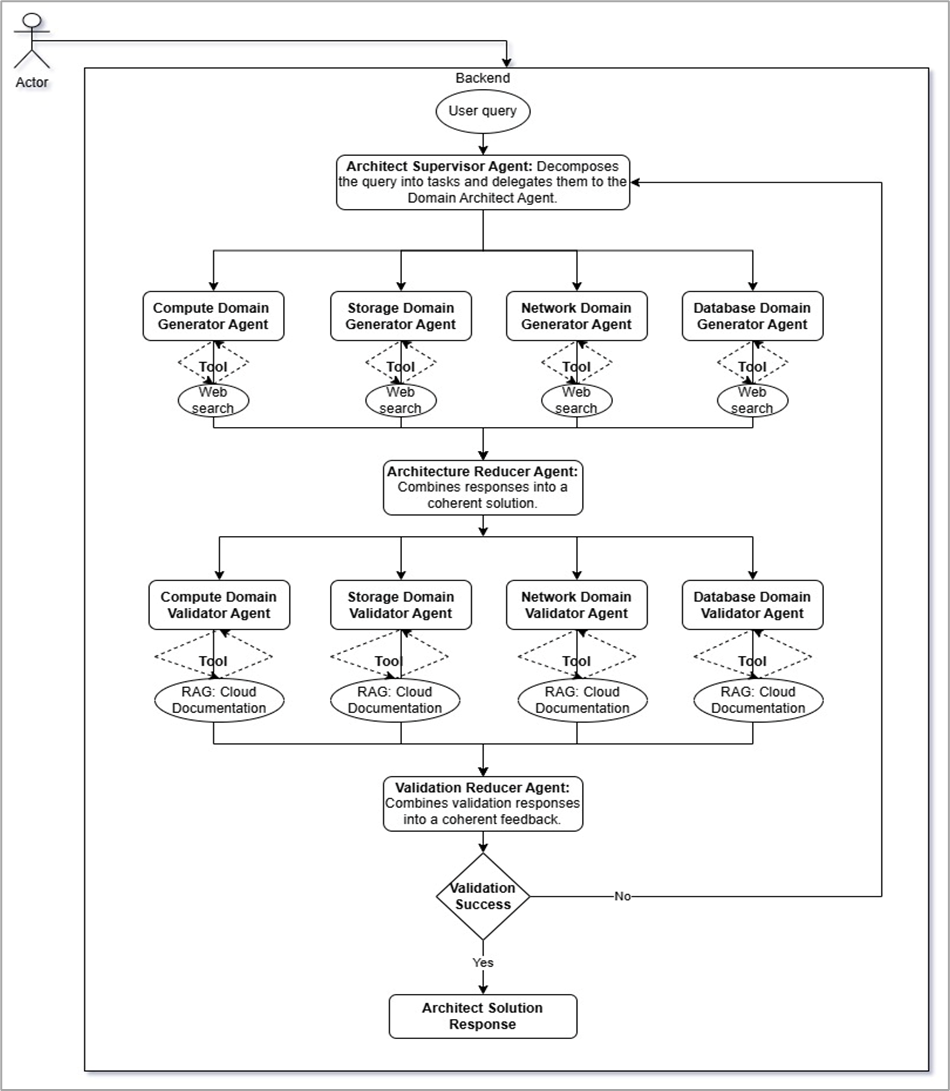
\includegraphics[width=11cm, height=12cm]{./figures/AgenticArchitect.png}
  \caption{Agent Framework: System Architecture Design}
  \label{fig:system_arch}
  \end{center}
\end{figure}


The architecture operates in five distinct phases managed by a graph-based state machine:

\subsection{Phase 1: Query Decomposition}

The \textbf{Architect Supervisor Agent} receives the user's natural-language problem statement and decomposes it into four structured domain tasks via a call to a \texttt{with\_structured\_output(TaskDecomposition)} LLM. Each task carries a precise description, key requirements, and expected deliverables. When running in a refinement iteration, the supervisor also receives the previous cycle's validation feedback and adjusts task definitions accordingly.

\subsection{Phase 2: Generation}

Four \textbf{Domain Architect Agents} (compute, network, storage, database) execute concurrently. Each agent operates a bounded ReAct loop \cite{yao2023react} equipped with two tools: a \textbf{Web Search} capability backed by the Google Serper API for real-time information, and a \textbf{RAG Search} capability backed by a provider-specific ChromaDB vector store. A configurable maximum number of tool-call rounds prevents unbounded token consumption.

\subsection{Phase 3: Architecture Synthesis}

The \textbf{Architect Synthesizer} waits for all four domain outputs and merges them into a single coherent architecture proposal. It resolves any cross-domain incompatibilities (for example, ensuring the network configuration exposes the correct ports for the proposed compute services) and produces both a structured component dictionary and a human-readable summary.

\subsection{Phase 4: Validation with Reranked RAG}

The \textbf{Validator Supervisor Agent} inspects the synthesized components and assigns targeted validation tasks to four \textbf{Domain Validator Agents}. Each validator exclusively uses the RAG tool, not web search, so that fact-checking is grounded in the curated documentation corpus rather than the open internet. Within the RAG tool, a two-stage retrieval protocol operates: ChromaDB performs an initial embedding-similarity search over a larger candidate pool (top-$k \times$ multiplier documents), and a FlashRank cross-encoder \cite{gao2023retrieval} subsequently rescores these candidates and returns only the top-$k$ highest-relevance passages.

\subsection{Phase 5: Validation Synthesis and Iteration}

The \textbf{Validation Synthesizer} consolidates domain-level feedback into a global assessment. The \texttt{iteration\_condition} function then inspects the state: if the minimum iteration count has not been reached, or if factual errors were reported and the maximum has not been exceeded, the graph routes back to the architect phase. Otherwise it routes to the final generator. This conditional edge is the mechanism that implements the Evaluator-Optimizer loop from Phase 1 \cite{anthropic2024agents}, now operating over subgraphs.

\subsection{Phase 6: Final Architecture Generation}

Once iteration terminates, the \textbf{Final Architecture Generator} compiles a deployment-ready document covering executive summary, domain-specific specifications, security controls, cost optimisation strategies, and Infrastructure-as-Code guidance. This output is persisted in the LangGraph state and returned to the UI.

\section{Model Selection Subsystem}

A persistent limitation of fixed-model architectures is that no single LLM dominates across all tasks: high-capability reasoning models process complex decomposition better, but their cost per token can be prohibitive for repetitive domain agent calls. The system introduces a two-tier model selection system.

A central model catalog defines available models across three providers (OpenAI GPT-5.4 family, Anthropic Claude~4.6 family, Google Gemini~3.1/2.5 family), tagged by tier (reasoning or execution). The \texttt{RuntimeContext} carries a base reasoning LLM and a base execution LLM set at service startup. Per-run overrides carried in the LangGraph state allow the UI to nominate different models for individual requests, ensuring that supervisors and synthesizers always use the appropriate reasoning-tier model while domain agents use the more cost-efficient execution-tier model.

\section{Algorithms and Techniques}

\subsection{Core Workflow: Evaluator-Optimizer}

The central workflow is a self-correcting "Evaluator-Optimizer" loop depicted in Figure \ref{fig:eval_workflow}, inspired by \cite{anthropic2024agents}. In each iteration, a Generator phase proposes an architectural solution, which a Validator phase critiques using RAG grounded in up-to-date vector database retrievals. The cycle continues until the solution passes all domain validation checks.

\begin{figure}[h]
    \centering
    \fbox{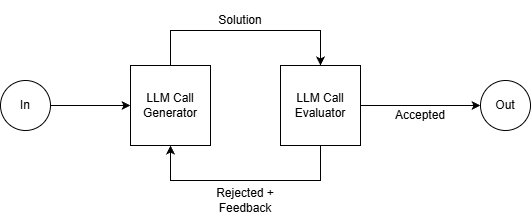
\includegraphics[width=0.9\textwidth]{./figures/Evalutor-Optimiser.drawio.png}}
    \caption[The Evaluator-Optimizer Workflow]{The Evaluator-Optimizer Workflow (Source: Adapted from \cite{anthropic2024agents})}
    \label{fig:eval_workflow}
\end{figure}

\subsection{Knowledge Base Construction (Data Pipeline)}

A reliable knowledge base underpins RAG-based validation. The pipeline is structured around four conceptual stages: (1)~\textbf{Data Collection}, gathering official documentation from each supported cloud provider through a combination of automated and manual methods; (2)~\textbf{Document Preprocessing}, converting multi-format sources (PDF, Markdown, DOCX) into uniformly structured text, stripping non-vectorisable content, and enriching each chunk with provenance metadata; (3)~\textbf{Embedding Generation}, transforming text chunks into dense semantic vectors using a locally hosted embedding model; and (4)~\textbf{Vector Indexing}, persisting those embeddings in a dedicated store that supports fast similarity-based lookup at validation time. The tools, libraries, chunking strategies, and hardware acceleration realising each stage are detailed in Chapter~4.

\section{Tools and Technologies}

The project prototype employs the following primary technologies and frameworks:

\begin{itemize}
    \item \textbf{Programming Language:} Python 3.11+ provides flexibility and robust libraries for AI and web integration.
    \item \textbf{Frontend Framework:} Next.js 15 with React 18 and the \texttt{@xyflow/react} library for interactive workflow graph visualization.
    \item \textbf{Agentic Framework:} LangGraph \cite{langgraph2024docs} enables cyclic, stateful multi-agent orchestration beyond linear pipelines.
    \item \textbf{LLM Orchestration:} LangChain \cite{langchain2024docs} and its Expression Language LCEL \cite{langchain2024lcel} streamline prompt management, chaining, and tool integration.
    \item \textbf{Local Embedding Service:} Ollama \cite{ollama2024web} with \texttt{nomic-embed-text} manages local LLM and embedding model.
    \item \textbf{Vector Database:} ChromaDB \cite{chromadb2024} indexes and enables fast semantic retrieval of vector embeddings crucial for RAG.
    \item \textbf{Live Data Integration:} Google Serper API is integrated to provide Generator Agents with real-time access to the latest cloud service documentation.
    \item \textbf{Graph Observability:} LangSmith is utilized to trace and debug the complex, non-deterministic execution paths of the cyclic multi-agent workflow.
    \item \textbf{Hardware Acceleration:} Apple Metal Performance Shaders (MPS) framework \cite{apple2024mps} accelerates embedding generation on Apple Silicon.
\end{itemize}

